\definecolor{matrizcol}{RGB}{80,240,120}
\definecolor{electroncol}{RGB}{120,80,220}

\tikzset{pics/electron/.style = {
    code = {
        \def\centerx{0}
        \def\centery{0}
        \draw[line width=0.25pt, ball color=electroncol] (\centerx,\centery) circle (1cm);
        \draw[fill=black, rounded corners=2pt] 
        (\centerx-0.4,\centery-0.1) rectangle ++(0.8,0.2);
    }
}}

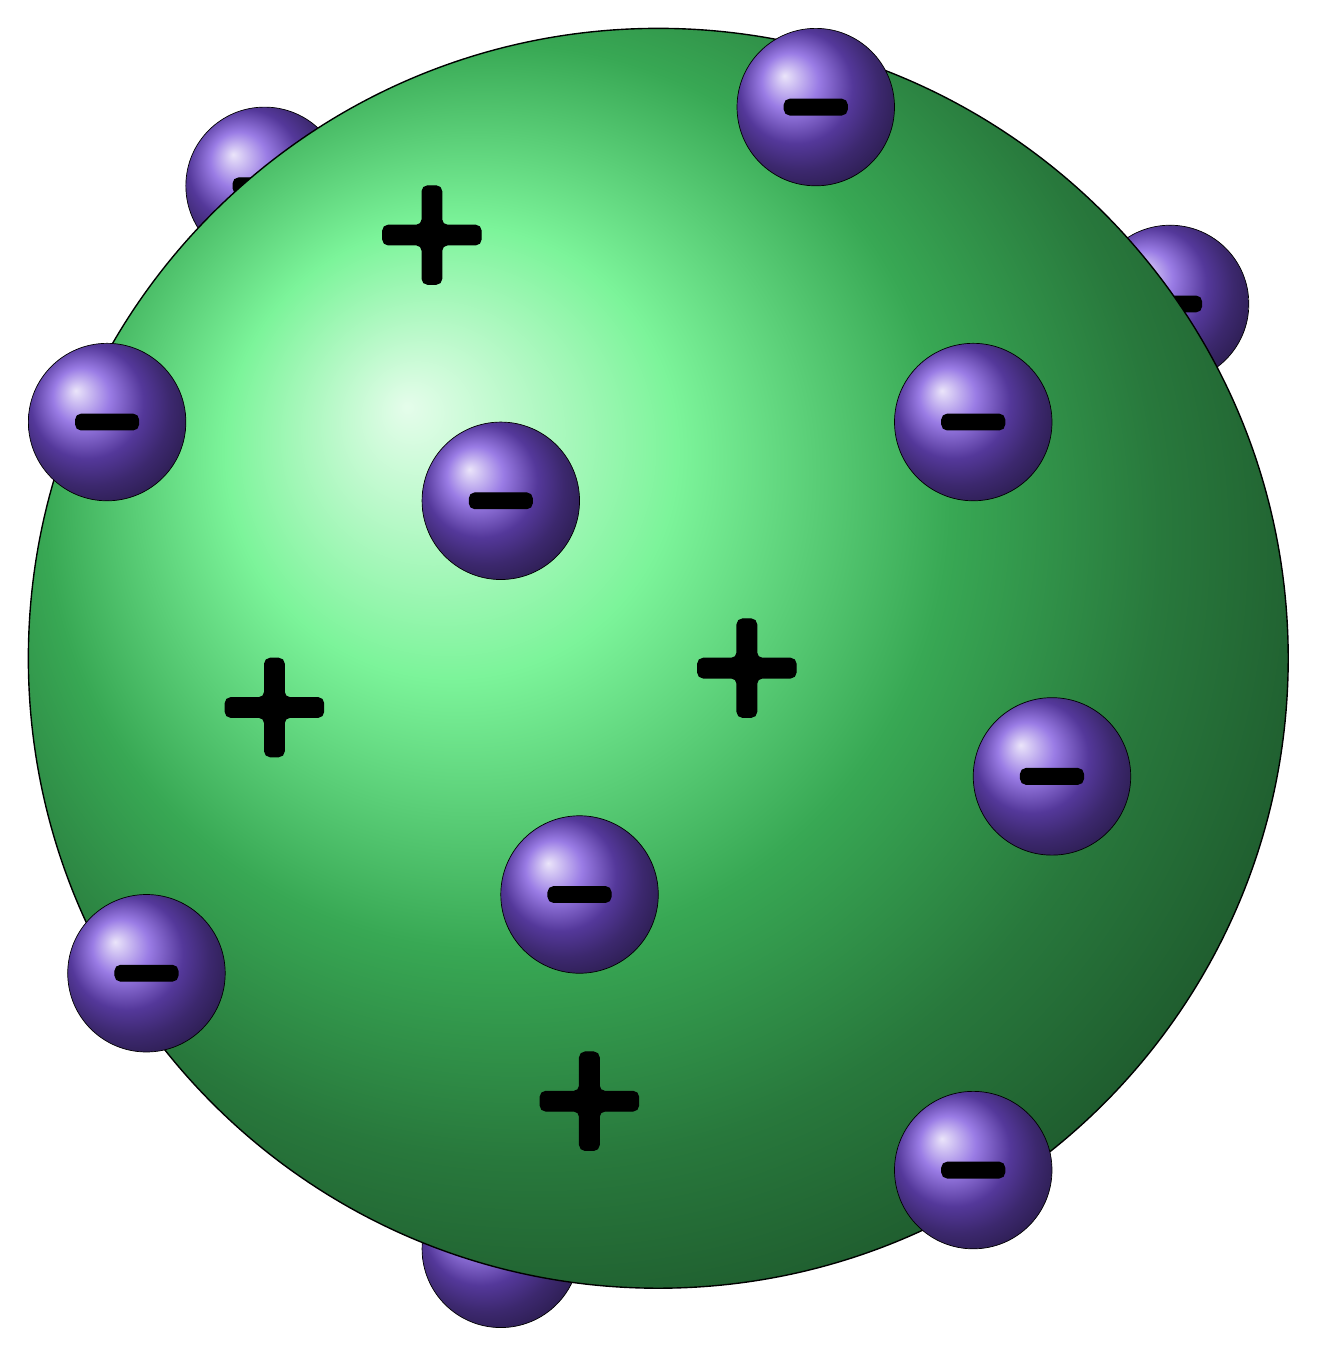
\begin{tikzpicture}[matriz/.style={line width=0.5pt, ball color=matrizcol}]

\foreach \coord in {
    {(-5,6)},
    {(6.5,4.5)},
    {(-2,-7.5)}
}{\path \coord pic {electron};}

\draw[matriz] (0,0) circle (8cm);

\foreach \coord in {
    {(-1,-3)},
    {(2,7)},
    {(5,-1.5)},
    {(-2,2)},
    {(4,3)},
    {(-7,3)},
    {(-6.5,-4)},
    {(4,-6.5)}
}{\path \coord pic {electron};}

\draw[fill=black, rounded corners=2pt] (-3,6) --++ (0.25,0) --++ (0,-0.5) --++ (0.5,0) --++ (0,-0.25) --++ (-0.5,0) --++ (0,-0.5) --++ (-0.25,0) --++ (0,0.5) --++ (-0.5,0) --++ (0,0.25) --++ (0.5,0) -- cycle;

\draw[fill=black, rounded corners=2pt] (-5,0) --++ (0.25,0) --++ (0,-0.5) --++ (0.5,0) --++ (0,-0.25) --++ (-0.5,0) --++ (0,-0.5) --++ (-0.25,0) --++ (0,0.5) --++ (-0.5,0) --++ (0,0.25) --++ (0.5,0) -- cycle;

\draw[fill=black, rounded corners=2pt] (1,0.5) --++ (0.25,0) --++ (0,-0.5) --++ (0.5,0) --++ (0,-0.25) --++ (-0.5,0) --++ (0,-0.5) --++ (-0.25,0) --++ (0,0.5) --++ (-0.5,0) --++ (0,0.25) --++ (0.5,0) -- cycle;

\draw[fill=black, rounded corners=2pt] (-1,-5) --++ (0.25,0) --++ (0,-0.5) --++ (0.5,0) --++ (0,-0.25) --++ (-0.5,0) --++ (0,-0.5) --++ (-0.25,0) --++ (0,0.5) --++ (-0.5,0) --++ (0,0.25) --++ (0.5,0) -- cycle;

\end{tikzpicture}